%===============================================================================
% $Id: ifacconf.tex 19 2011-10-27 09:32:13Z jpuente $  
% Template for IFAC meeting papers
% Copyright (c) 2007-2008 International Federation of Automatic Control
%===============================================================================
\documentclass{ifacconf}

\usepackage{graphicx}      % include this line if your document contains figures
\usepackage{natbib}        % required for bibliography
\usepackage{amsmath}
%===============================================================================
\begin{document}
\begin{frontmatter}

\title{Grupo 3 - Módulo 2 - Maglev} 
% Title, preferably not more than 10 words.

%\thanks[footnoteinfo]{Sponsor and financial support acknowledgment
%goes here. Paper titles should be written in uppercase and lowercase
%letters, not all uppercase.}

\author[First]{Felipe Nery Barcelos Araújo (2020021190)} 
\author[First]{Gustavo Vieira Barbosa (2020021352)} 
\author[First]{Matheus Marques Gonçalves de Paula (2020068995)}

\address[First]{
  Engenharia de Controle e Automação,\\ Universidade Federal de Minas Gerais, MG \\
   (e-mails: felipenery@ufmg.br, gustavovbarbosa@ufmg.br, mmgp@ufmg.br)
}

%Escrever um resumo do documento aqui, não pode ultrapassar 250 palavras
\begin{abstract}               
Relatório do controle de posição de uma massa levitada por um eletroima
\end{abstract}

%Escrever até 5 palavras chave do relatório aqui
\begin{keyword}
maglev, controle, posição, levitação, eletroima
\end{keyword}

\end{frontmatter}

%===============================================================================

\section{Introdução}

A levitação magnética, é uma tecnologia em que utiliza forças magnéticas para suspender e controlar a posição de
objetos metálicos, como uma esfera de aço, sem a necessidade de contato físico com superfícies. Um exemplo notável dessa aplicação é a levitação de uma esfera
de aço por meio da força magnética gerada por um eletroímã, que será abordado nesse relatório por meio da planta Maglev da \textit{Feedback}. Tal controle tem importância significativa 
tanto na sociedade como na indústria, oferecendo uma ampla gama de benefícios, desde sistemas de transporte de alta velocidade até aplicações em pesquisa e desenvolvimento.

Ao longo desse relatório será visto um estudo focado no controle de posição de uma esfera de aço por meio de forças magnéticas 
gerada por um eletroímã, como mostra a figura \ref{fig:planta_padrao}, um problema
clássico de controle de sistemas magnéticos. 

\begin{figure}[!htb]
  \begin{center}
  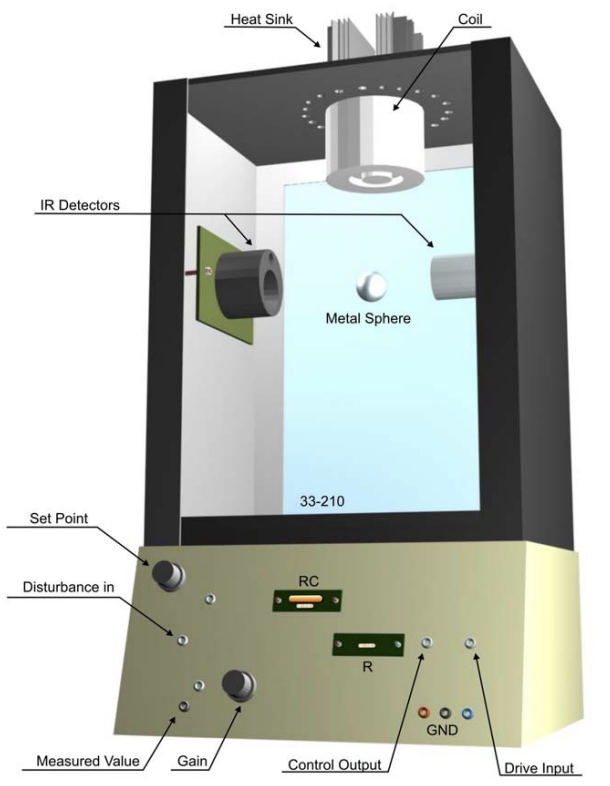
\includegraphics[width=6.4cm]{figures/planta_padrao.png}    % The printed column width is 8.4 cm.
  \caption{Figura da planta real estudada, levitador magnético (Maglev). Fonte: Autoral} 
  \label{fig:planta_padrao}
  \end{center}
\end{figure}

Com isso, nas seções subsequentes, exploraremos em detalhes a modelagem matemática do sistema
maglev, bem como o fundamento do controle utilizado e demonstrações práticas.

\section{Descrição da planta e especificação do desempenho desejado}

O controle a ser realizado visa, inicialmente, controlar a posição de uma esfera de aço bem como tornar o sistema estável (deixando-a parada) com erro nulo para entrada de degrau, 
%CONFIRMAR ISSO DO TEMPO DE ACOMADAÇÃO E SOBRESSINA.
A planta a ser estudada envolve além da esfera de aço, um eletroímã, o qual irá gerar um campo magnético que
consequentemente irá impor uma força eletromagnética sobre a esfera fazendo-a levitar com um controle preciso de posição.


\section{Modelagem matemática e validação do modelo}

\subsection{Modelagem do Sensor}

A variável quantificada pelo sensor corresponde à distância,
sendo que sua resposta resultante é expressa em termos de tensão.
Neste contexto, surge a necessidade de um modelo que estabeleça a
relação entre a resposta em tensão gerada pelo sensor e a distância
efetivamente medida por este último. Devido à proporcionalidade
das variáveis, a relação entre elas pode ser expressa pela seguinte
função:
\begin{equation}
    y = ax + b
\end{equation}
onde:
\begin{itemize}
    \item y - resposta do sensor em volts [V]
    \item x - distância medida em metros [m]
    \item a - constante de ganho do sensor em volts por metro [V/m]
    \item b - constante de offset do sensor em volts [V]
\end{itemize}

\subsection{Modelagem da Planta}

Inicialmente, procedemos com uma análise das forças atuantes
no sistema em questão. A força exercida pela bobina é formulada
mediante a seguinte expressão matemática:
\begin{equation}
    \vec{F_b} = k \frac{i^2}{x^2}
\end{equation}

\noindent onde $i$ representa a intensidade da corrente elétrica, $x$ denota adistância entre o objeto e a bobina, e $k$ representa um coeficiente intrínseco ao circuito elétrico. Paralelamente, a força gravitacional que age sobre um corpo é definida como:

\begin{equation}
    \vec{F_g} = mg
\end{equation}

\noindent onde $m$ corresponde à massa do corpo em questão, e $g$ representa a aceleração devida à gravidade. Em concordância comos princípios da segunda lei de Newton, podemos estabelecer o
seguinte resultado:

\begin{equation}
    m\ddot{x} = mg - k \frac{i^2}{x^2}
\end{equation}

\begin{equation}
    f(x,i) = \ddot{x}_2 = g - \frac{k}{m} \frac{i^2}{x^2}
    \label{eq:eqdif}
\end{equation}

\subsection{Linearização}

A teoria de controle linear parte do princípio de que a planta
possui comportamento linear. Mas nem sempre isto é
verdade. Contudo, para toda função bem comportada em torno de
um ponto fixo, para variações pequenas, curva pode ser aproximada por uma reta que passa pelo ponto fixo. Novas equações podem ser obtidas a partir de (7) e (9) de modo a se obter a dinâmica para pequenas variações. Por este motivo as seguintes variáveis são definidas:

\begin{equation}
    \delta x = x - x_{eq}
\end{equation}
\begin{equation}
    \delta i = i - i_{eq}
\end{equation}
\begin{equation}
    \delta y = y - y_{eq}
\end{equation}

\noindent onde $x$, $i$ e $y$ são as variáveis originais, $x_{eq}$, $i_{eq}$ e $y_{eq}$ são valores que a planta assume quando está em uma condição de equilíbrio e $\delta x$, $\delta i$ e $\delta y$ as variações em torno do ponto de equilíbrio. Vale ressaltar que o ponto de equilíbrio escolhido deve ser o mais próximo possível das especificações de desempenho desejado, ou seja, os valores que fazem a esfera flutuar a 9 mm, pois fora do ponto de equilíbrio os comportamentos não lineares são mais evidentes. Encontra-se os pontos de equilíbrio igualando a equação \ref{eq:eqdif} a 0.

\begin{equation}
    \ddot{x}_2 = g - k \frac{i^2}{x^2} = 0 \rightarrow i = \sqrt{\frac{mg}{k}}x
\end{equation}
Quaisquer combinações de $i$ e $x$ que satisfaçam a relação anterior são considerados pontos de equilíbrio. Os valores de $m$ e $k$ não são definidos separadamente, mas sim através da seguinte relação:
\begin{equation}
    \frac{k}{m} = 1,2415 \cdot 10^{-3}
\end{equation}
\noindent que é inerente ao sistema. A aceleração da gravidade é tomada por $g = 9,81 \; m/s^2$. Sendo assim, a corrente de entrada para uma saída de equilíbrio $x_o = 9\;mm$ é:
\begin{equation}
    i_o = \sqrt{\frac{9,81\;m/s^2}{1,2415 \cdot 10^{-3}}} \cdot 0,009\;m
\end{equation}
\begin{equation}
    i_o = 0,8\;A
\end{equation}
Portanto, a entrada e a saída de equilíbrio estipulados são $i_o = 0,8\;A$ e $x_o = 0,009\;m$, respectivamente. Neste ponto, o sistema é linearizado, deslocando-se o referencial, de modo que sua nova origem coincida com este ponto. O modelo linearizado da planta, então, é dado por:
\begin{equation}
    \ddot{x} = -[K_i i + a_x x]
    \label{eq:linear}
\end{equation}
onde $K_i$ e $a_x x$ são coeficientes dados por:
\begin{equation}
    K_i = [\frac{\partial}{\partial i}f(x,i)]_{x = x_o, i = i_o}
\end{equation}
\begin{equation}
    a_x = [\frac{\partial}{\partial x}f(x,i)]_{x = x_o, i = i_o}
\end{equation}
Tomando as derivadas parciais e aplicando o ponto de operação, tem-se:
\begin{equation}
    K_i = \frac{-2ki_o}{mx_o^2} = \frac{-2\cdot1,2415 \cdot 10^{-3}\cdot 0,8\;A}{(0,009\;m)^2} = -24,5250
\end{equation}
\begin{equation}
    a_x = \frac{2ki_o^2}{mx_o^3} = \frac{2\cdot1,2415 \cdot 10^{-3}\cdot (0,8\;A)^2}{(0,009\;m)^3} = 2180
\end{equation}

Aplicando a transformada de Laplace ao modelo linearizado em \ref{eq:linear}, tem-se a seguinte função de transferência:
\begin{equation}
    s^2X(s) = -K_i I(s) - a_x X(s)
\end{equation}
\begin{equation}
    G(s) = \frac{X(s)}{I(s)} = \frac{-K_i}{s^2+a_x}
    \label{eq:FT1}
\end{equation}

Entretanto, a entrada do sistema, na prática, é dada por tensão. Essa relação é descrita por:
\begin{equation}
    i(t) = k_1u(t)
\end{equation}
\noindent onde $k_1$ é uma constante de proporcionalidade entre a tensão e a corrente do circuito e depende inteiramente das características físicas do mesmo. A equação anterior, no domínio de Laplace, se torna:
\begin{equation}
    I(s) = k_1U(s)
    \label{eq:tensaocorrentelaplace}
\end{equation}
Substituindo \ref{eq:tensaocorrentelaplace} em \ref{eq:FT1}, tem-se:
\begin{equation}
    G(s) = \frac{X(s)}{k_1U(s)} = \frac{-k_1K_i}{s^2+a_x}
    \label{eq:FT2}
\end{equation}

Por fim, a saída da planta, na prática, é dada por tensão, através da relação:
\begin{equation}
    v(t) = k_sx(t)
\end{equation}
que, em Laplace, é:
\begin{equation}
    V(s) = k_sX(s)
    \label{eq:tensaosaidalaplace}
\end{equation}
Substituindo \ref{eq:tensaosaidalaplace} em \ref{eq:FT2}, tem-se:
\begin{equation}
    G(s) = \frac{V(s)}{U(s)} = \frac{-k_sk_1K_i}{s^2+a_x}
\end{equation}
Os valores das constantes são:
\begin{equation}
    k_1 = 1,05\; A/V
\end{equation}
\begin{equation}
    k_s = 143,48\; V/m
\end{equation}
\noindent e foram obtidos pelo diagrama de simulação da planta.
Ao final, a função de transferência que descreve o comportamento linear da planta em torno do ponto de operação estipulado em $x_o = 0,009\;m$ é:
\begin{equation}
    G(s) = \frac{3695}{s^2 - 2180}
    \label{eq:FTFINAL}
\end{equation}

\subsection{Validação do Modelo}
O modelo obtido não é estável e, portanto, não é possível aplicar uma entrada de tensão sem que a saida divirja. Sendo assim, o modelo será validado juntamente com um controle PD. Para o mesmo, o lugar das raízes da planta $G(s)$ foi analizado a fim de estipular um controlador PD do tipo:
\begin{equation}
    C(s) = K_d(s+\frac{K_p}{K_d})
\end{equation}
\noindent onde $K_d$ é o ganho do controlador e $\frac{K_p}{K_d}$ é o zero do mesmo. O lugar das raízes da planta está presente na figura abaixo.

[COLOCAR LUGAR DAS RAIZES TÁ NO DESKTOP DO GUSTAVO]

Sendo assim, a fim de estabilizar a planta, foi estipulado um zero em $s = -20$ e um ganho de 0,2, que resultou no seguinte lugar das raízes, com o deslocamento do polo instável para $s = -17,5$. O outro polo é negativo, então, para fins de validação, já está satisfatório.

[COLOCAR LUGAR DAS RAIZES CORRIGIDO TÁ NO DESKTOP DO GUSTAVO]

Portanto, tem-se:
\begin{equation}
    K_i = 0,2
\end{equation}
\begin{equation}
    \frac{K_p}{K_i} = 20 \rightarrow K_p = 4
\end{equation}

\section{Projeto do controlador}
 
\subsection{Parâmetros do PID}
Primeiramente, foi utilizado a modelagem do Maglev para encontrar os melhores valores de Kp, Ki e Kd para o controlador PID.
Para isso, foi utilizado a ferramenta \textit{sisotool} do \textit{matlab} para posicionamento dos dois zeros e do integrador no sistema em malha fechada.
Utilizando a abordagem de controle clássica do lugar das raízes, os zeros e o integrador foram adicionados e o ganho foi variado para encontrar o melhor posicionamento 
dos polos do sistema em malha fechada, como mostrado pela Figura \ref{fig:pid_inicial} . A lei de controle encontrada pelo método foi:

\begin{equation}
  C(s) = 4 + \frac{20}{s} + 0.2s
  \label{equa: controle inicial}
\end{equation}

\begin{figure}[!htb]
  \begin{center}
  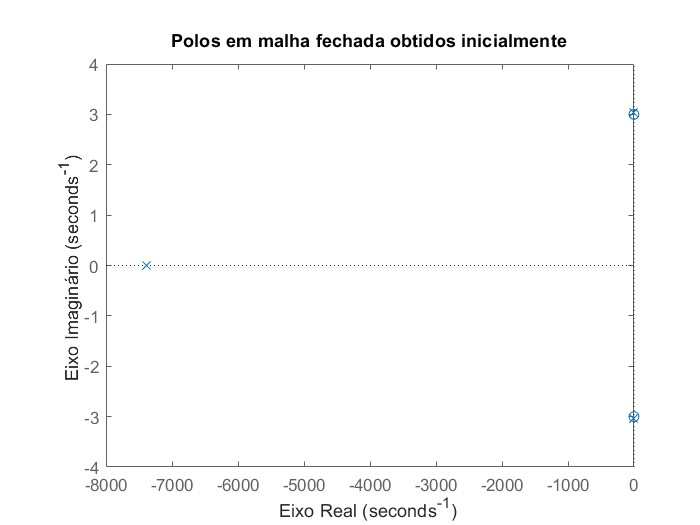
\includegraphics[width=8.4cm]{figures/lei pid inicial.jpg}    % The printed column width is 8.4 cm.
  \caption{Posicionamento dos polos em malha fechada do sistema com o controle PID. Fonte: autoral, produzido com \textit{matlab}} 
  \label{fig:pid_inicial}
  \end{center}
\end{figure}

Contudo, ao testar esses parâmetros no modelo real, percebeu-se que ao passar 15 segundos do início da simulação(momento em que a ação integral entra em ação),
a bola de metal caía ou era atraída até encostar no ímã, isso mostra a facilidade com que o sistema entrava em instabilidade, sendo que isso não era previsto pelo modelo matemático. Esse 
potencial de instabilidade pode ser visto pela Figura \ref{fig:pid_inicial}, em que há pouca margem de fase para o sistema, porque os polos complexos conjugados estão muito perto do eixo 
real e isso torna o sistema mais sensível à se tornar instável.

À partir disso, chegou-se à conclusão de tentar encontrar o parâmetro $Ki$ heurísticamente, pois como mostrado pela lei de controle na Equação \ref{equa: controle inicial}, esse valor era bem mais elevado que os demais. 
Fazendo esse estudo das variações do parâmetro, encontrou-se o melhor valor para o ganho integrativo, como mostrado pela nova lei de controle na Equação \ref{equa: controle ajustado}. A nova lei de controle permitiu que 
o sistema se mantivesse mais equilibrado na região de referência estabelecida, em contrapartida o sistemas continuava se tornando instável com o passar do tempo e com isso tornou-se necessária 
a aplicação de um filtro para melhorar a ação de controle.

\begin{equation}
  C(s) = 4 + \frac{2}{s} + 0.2s
  \label{equa: controle ajustado}
\end{equation}

\begin{figure}[!htb]
  \begin{center}
  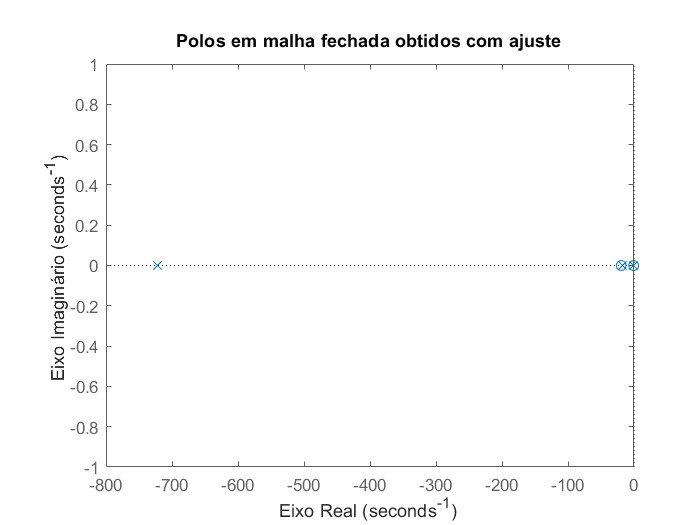
\includegraphics[width=8.4cm]{figures/lei pid ajuste.jpg}    % The printed column width is 8.4 cm.
  \caption{Posicionamento dos polos em malha fechada do sistema com o controle PID ajustado. Fonte: autoral, produzido com \textit{matlab}} 
  \label{fig:pid_ajustado}
  \end{center}
\end{figure}

Ao longo do estudo da resposta da posição da bola metálica no sistema, ficou clara a influência da variação da referência na ação de controle, sendo que variações abruptas são 
intensificadas pelo termo derivativo, por causa da sua tendência em amplificar ruídos de alta frequência(a variação abrupta do sinal de referência implica em um sinal com componentes 
de alta frequência). Outro ponto importante, é que a ação proporcional amplifica a diferença entre as referências , o que também contribui para a má qualidade do sinal de controle.

\begin{figure}[!htb]
  \begin{center}
  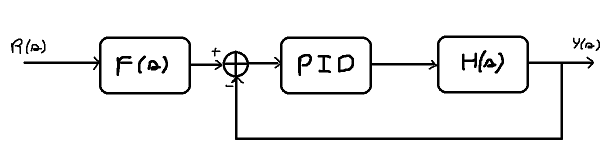
\includegraphics[width=8.4cm]{figures/Diagrama filtro.png}    % The printed column width is 8.4 cm.
  \caption{Diagrama de blocos do sistema com o filtro na parte externa. Fonte: autoral} 
  \label{fig:diagrama_filtro}
  \end{center}
\end{figure}

Analisando esses aspectos, chegou-se à conclusão de que o filtro ideal a ser aplicado é o filtro de referência, mostrado pela figura \ref{fig:diagrama_filtro}, que introduz parâmetros $b$ e $c$ para controlar o efeito das ações 
proporcional e derivativa, respectivamente. Esse filtro é implementado depois da referência e antes do nó de soma e possui a forma mostrada pela Equação \ref{equa: filtro}, para assim deixar 
a ação de controle com o aspecto desejado e representado pela Equação \ref{equa: controle filtrado}.

\begin{equation}
  F(s) = \frac{1+bsT_{i}+cs^2T_{i}T_{d}}{1+sT_{i}+s^2T_{i}T_{d}}
  \label{equa: filtro}
\end{equation}

\begin{equation}
  U(s) = K_{p}(bR(s)-Y(s)) + K_{i}\frac{E(s)}{s} + K_{d}s(cR(s)-Y(s))
  \label{equa: controle filtrado}
\end{equation}

Vale ressaltar que os parâmetros do PID mostrados pela Equação \ref{equa: controle ajustado} foram utilizados para encontrar os termos $Td$ e $Ti$ do filtro de referência e a relação entre esses parâmetros 
é descrita pelas equações abaixo:

\begin{equation*}
  T_{i} = \frac{K_{p}}{K_{i}}
  \label{equa: ti}
\end{equation*}

\begin{equation*}
  T_{d} = \frac{K_{d}}{K_{p}}
  \label{equa: td}
\end{equation*}

Por fim, os parâmetros $b$ e $c$ foram determinados empiricamente, levando em conta a teoria explicada e após alterá-los e testar o sistema sucessivamente para a mesma bolinha esférica, 
chegou-se no valor 0,25 e 0,4 para os parâmetros $b$ e $c$, respectivamente. Com isso o filtro implementado no sistema possui a seguinte forma:

\begin{equation}
  F(s) = \frac{0.04s^2+0.5s+1}{0.1s^2+2s+1}
  \label{equa: filtro completo}
\end{equation}


\section{Resultados experimentais em malha fechada}

\begin{figure}[!htb]
  \begin{center}
  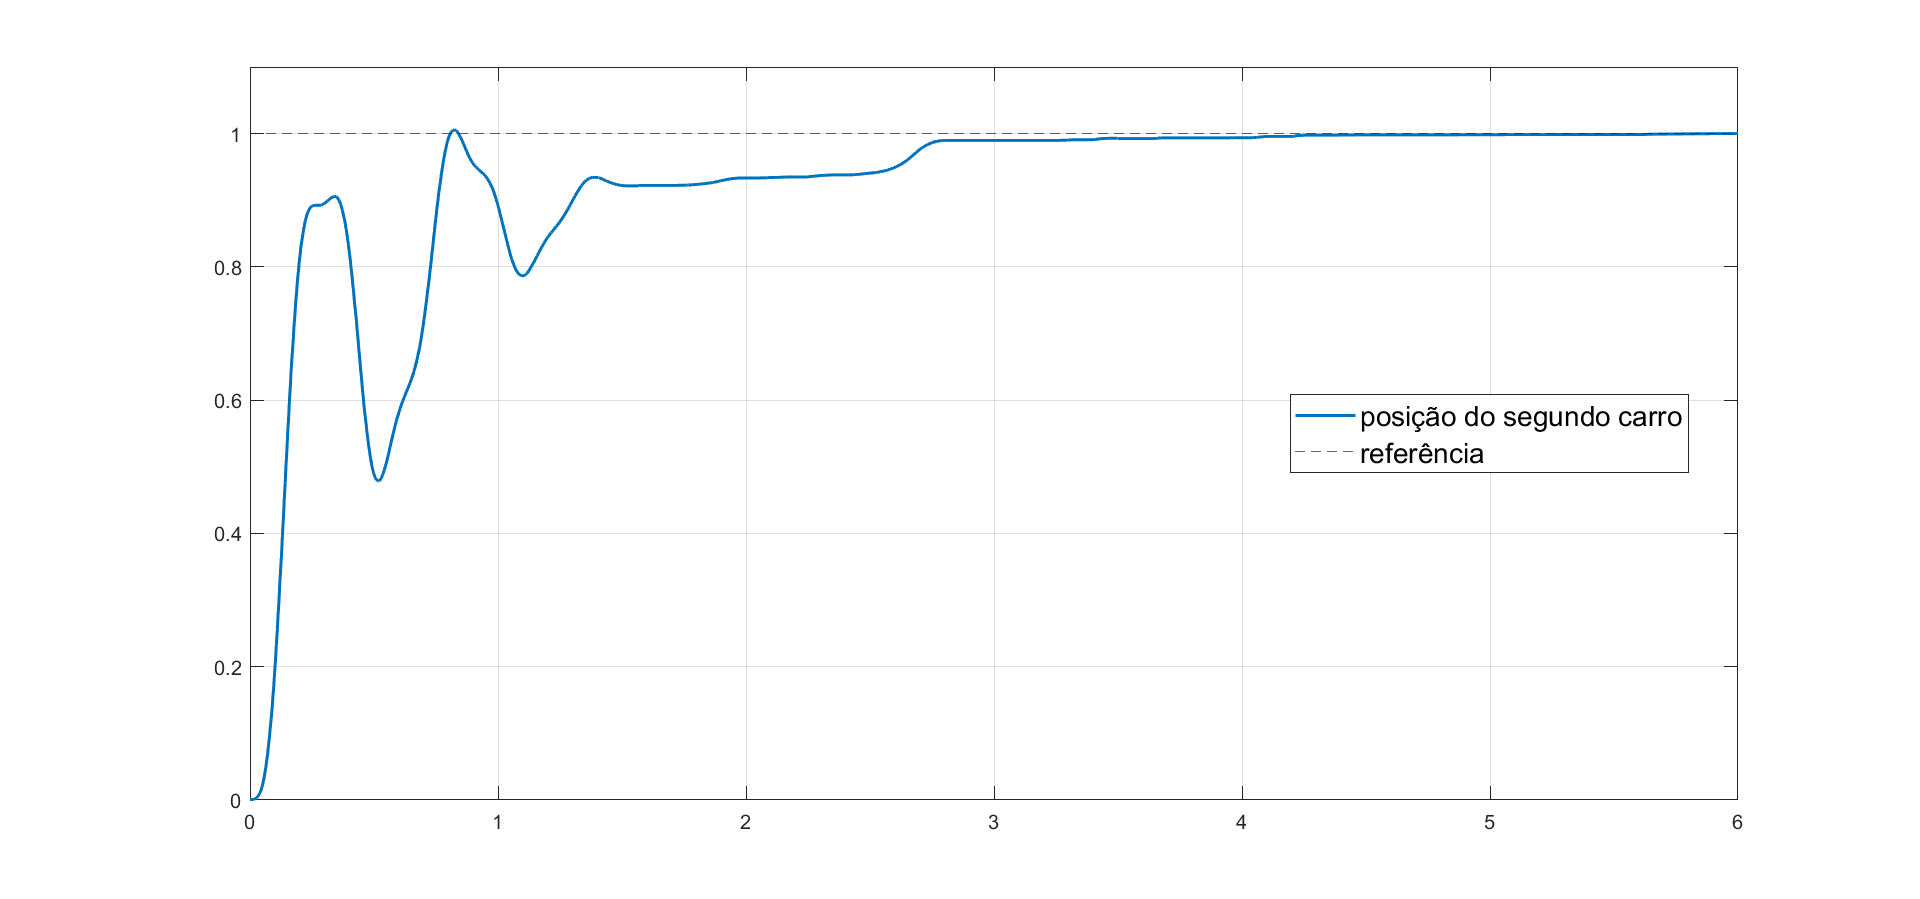
\includegraphics[width=8.4cm]{figures/resultado_teste1.png}    % The printed column width is 8.4 cm.
  \caption{Resposta a onda quadrada com A=5,29mm e F=0,1Hz, e filtro com b=0,25 e c=0,4. Fonte: autoral, produzido com \textit{matlab} por meio dos dados coletados na planta.} 
  \label{fig:teste1}
  \end{center}
\end{figure}

\begin{figure}[!htb]
  \begin{center}
  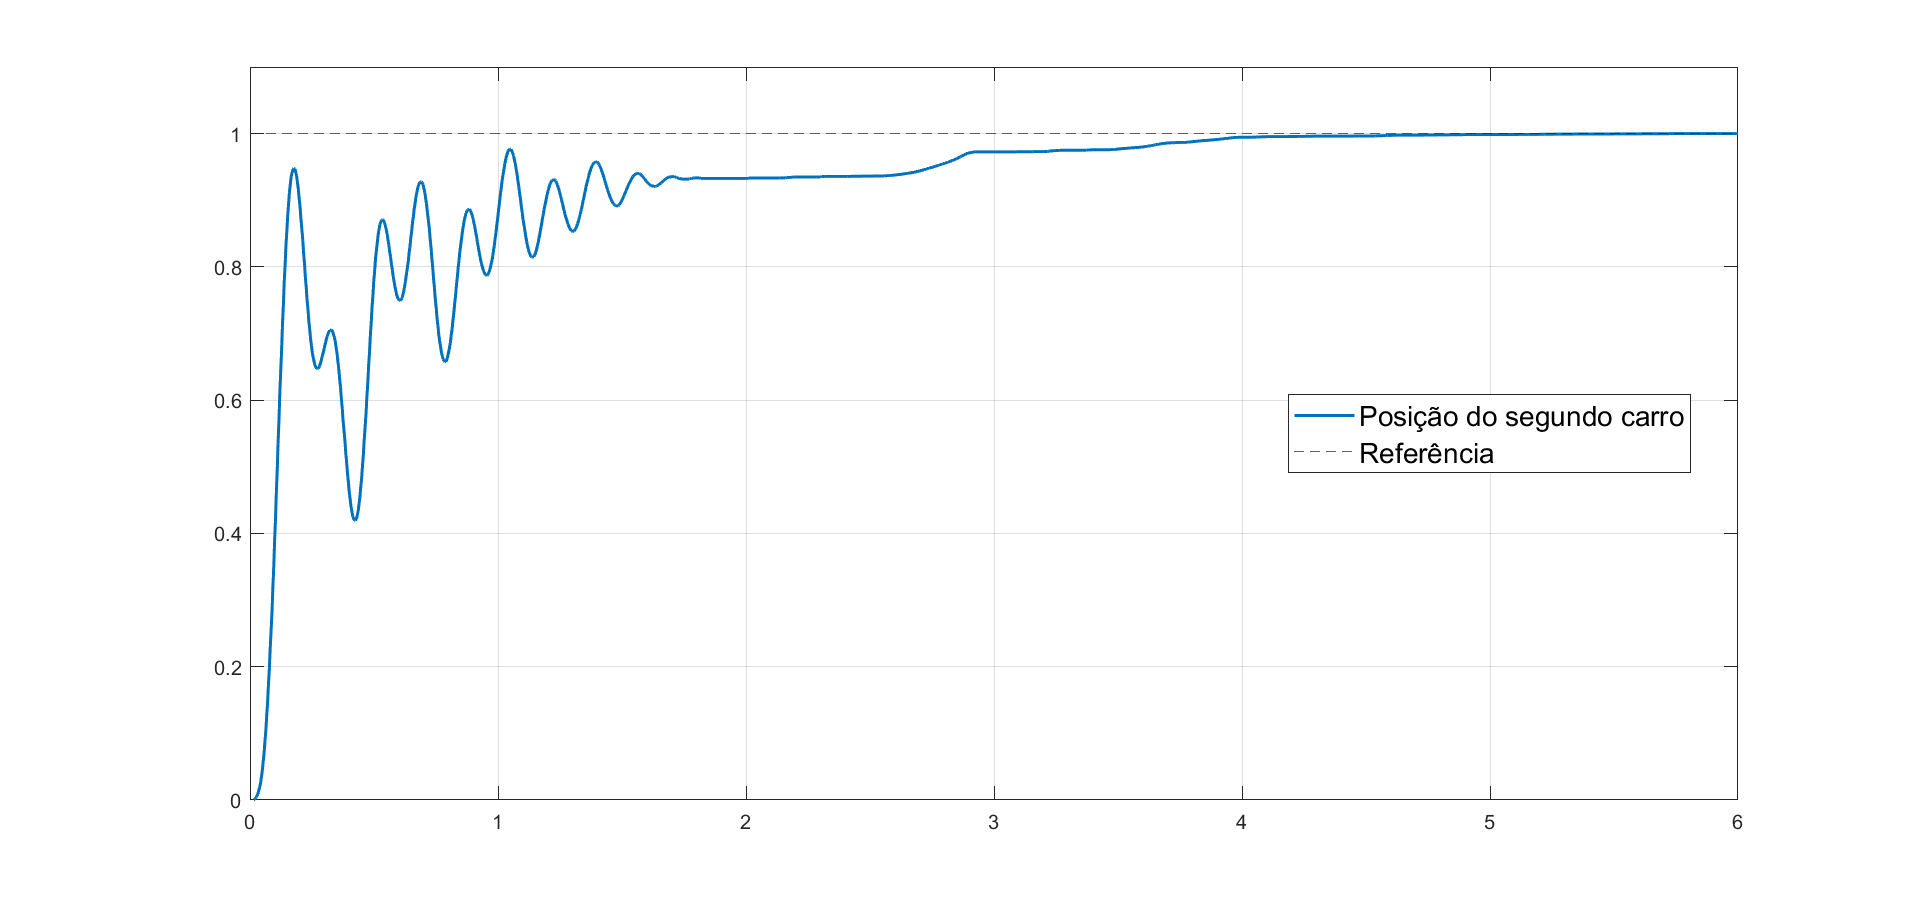
\includegraphics[width=8.4cm]{figures/resultado_teste2.png}    % The printed column width is 8.4 cm.
  \caption{Resposta a onda quadrada com A=5,29mm e F=0,1Hz, e filtro com b=0,15 e c=0,4. Fonte: autoral, produzido com \textit{matlab} por meio dos dados coletados na planta.} 
  \label{fig:teste2}
  \end{center}
\end{figure}

\begin{figure}[!htb]
  \begin{center}
  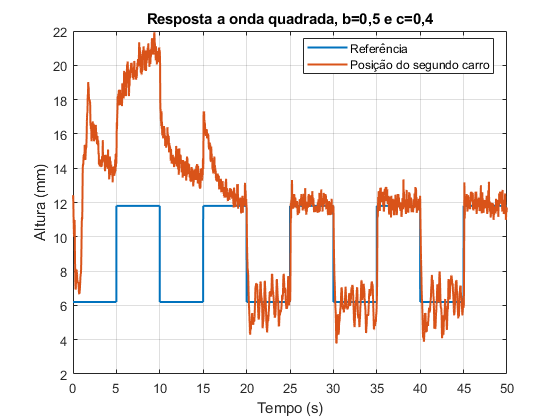
\includegraphics[width=8.4cm]{figures/resultado_teste3.png}    % The printed column width is 8.4 cm.
  \caption{Resposta a onda quadrada com A=5,29mm e F=0,1Hz, e filtro com b=0,5 e c=0,4. Fonte: autoral, produzido com \textit{matlab} por meio dos dados coletados na planta.} 
  \label{fig:teste3}
  \end{center}
\end{figure}

\begin{figure}[!htb]
  \begin{center}
  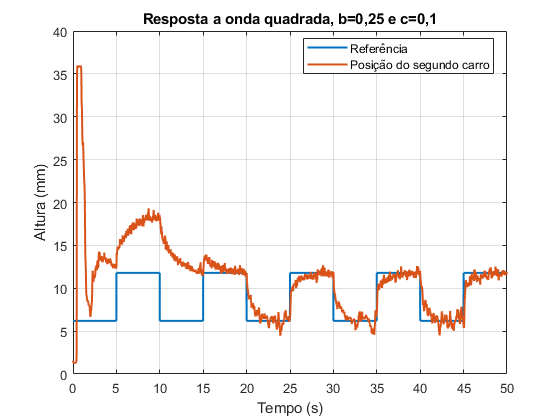
\includegraphics[width=8.4cm]{figures/resultado_teste4.png}    % The printed column width is 8.4 cm.
  \caption{Resposta a onda quadrada com A=5,29mm e F=0,1Hz, e filtro com b=0,25 e c=0,1, carro 1 e 2 com 4 pesos. Fonte: autoral, produzido com \textit{matlab} por meio dos dados coletados na planta.} 
  \label{fig:teste4}
  \end{center}
\end{figure}

\begin{figure}[!htb]
  \begin{center}
  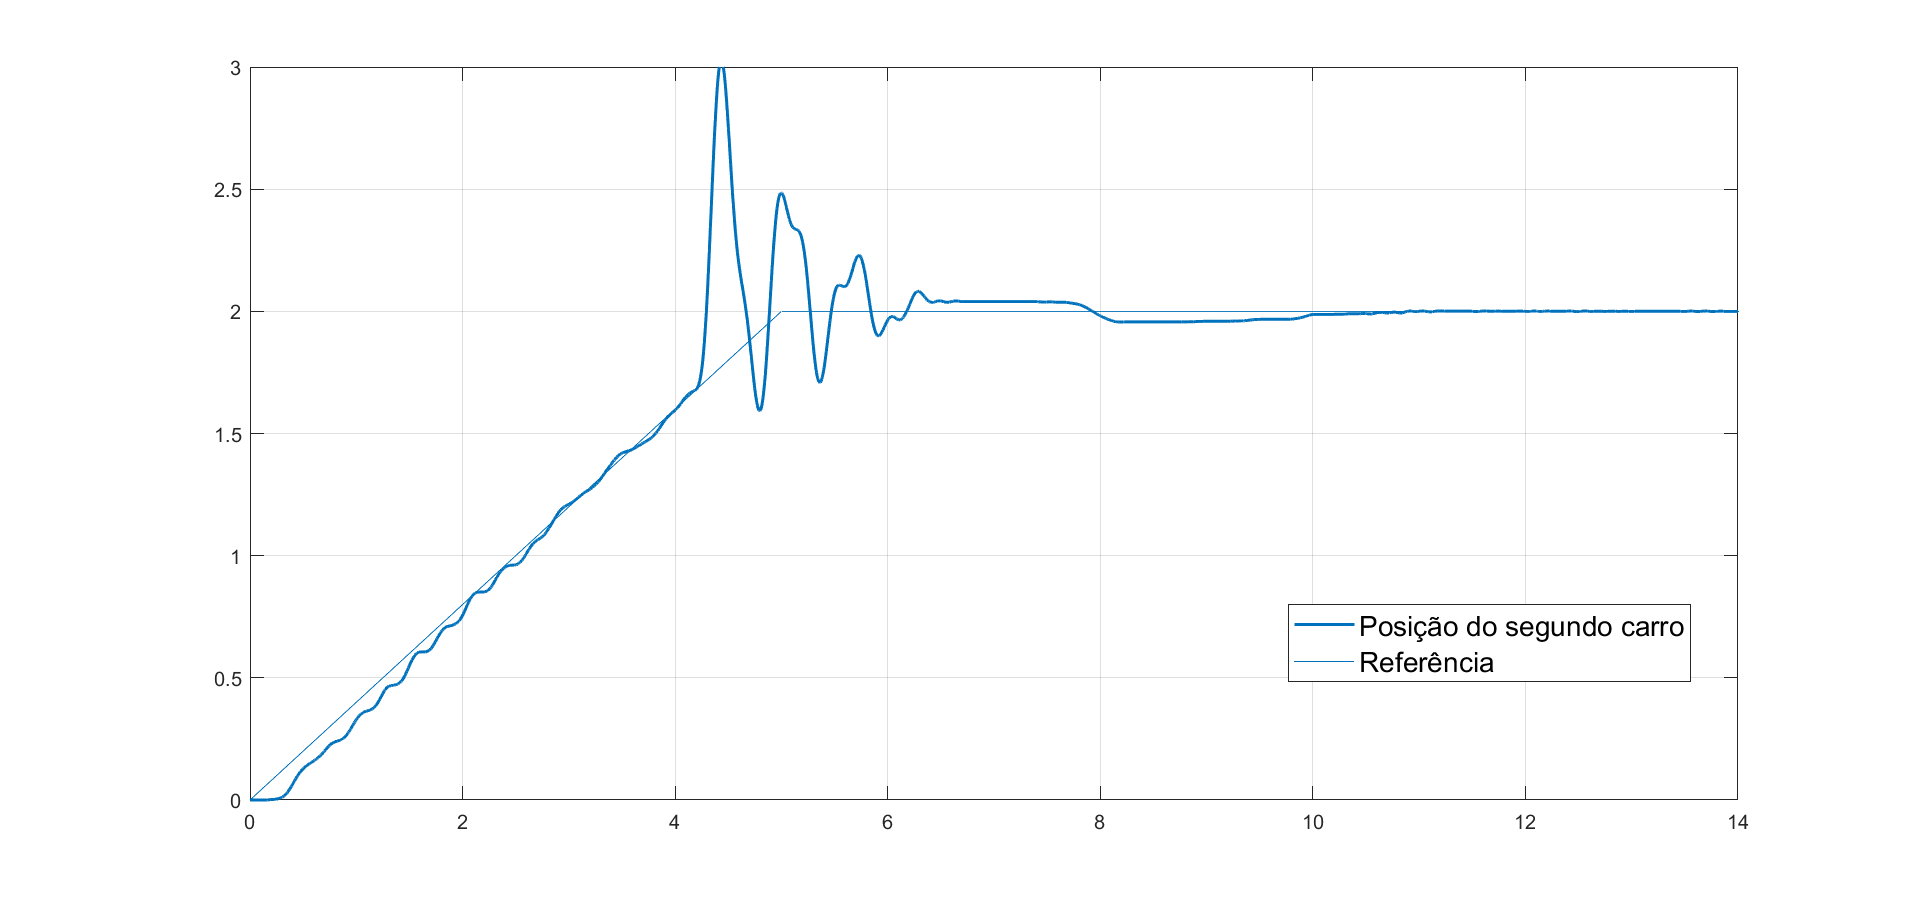
\includegraphics[width=8.4cm]{figures/resultado_teste5.png}    % The printed column width is 8.4 cm.
  \caption{Resposta a onda quadrada com A=5,29mm e F=0,1Hz, e filtro com b=0,25 e c=0,8, carro 1 e 2 com 4 pesos. Fonte: autoral, produzido com \textit{matlab} por meio dos dados coletados na planta.} 
  \label{fig:teste5}
  \end{center}
\end{figure}

Analisando os testes exemplificados, vemos que no início a resposta é muito afetada pelo fato da planta exigir que a esfera de aço parte de uma posição favorável para a força magnética atuar, com isso a esfera 
era colocada manualmente e, portanto, sujeita a diversos erros humanos de precisão como foi visto, mas após a esfera ser posicionada ela entra para o controle da planta.
Ademais, quando a esfera entra na região de controle, é visto que o controle foi eficaz, pois foi capaz de atingir a referência de forma rápida, mas oscilava bem pouco em torno dela devido as características
intrínsecas a planta. 

\section{Conclusão}

Por fim, vale ressaltar que o projeto envolveu o estudo da modelagem e controle de uma planta linear e serviu de base para o estudo prático das teorias de controle estudadas ao longo de disciplinas de semestres anteriores. A modelagem envolveu o uso de uma abordagem fenomenológica para a decomposição das forças do sistema e a partir disso os parâmetros da planta foram encontrados com a realização de testes envolvendo a troca de molas, pesos e a fixação dos carrinhos. Depois de modelar o sistema, foi desenvolvido um controlador com base no método do lugar das raízes com o \textit{software} \textit{Matlab} e com isso os parâmetros da resposta foram aprimorados para maior confiabilidade do modelo. Com isso, os parâmetros do PID foram implementados de forma discreta no controlador do sistema massa mola e diversos testes com entradas diferentes foram feitos.  

\section{Referências}

\begin{itemize}
  \item Notas de aula
  \item Manual da planta
\end{itemize}

\end{document}